\documentclass[12pt,a4paper]{article}
\usepackage[utf8]{inputenc}
\usepackage{amsmath, amssymb, amsfonts}
\usepackage{geometry}
\geometry{margin=2.5cm}
\usepackage{hyperref}
\usepackage{pgfplots}
\usepackage{fancyhdr}
\usepackage{graphicx}
\usepackage{listings}
\usepackage{listing}
\usepackage{titlesec}
\titleformat{\section}
  {\normalfont\Large\bfseries\centering}  % Format: font size, bold, centered
  {\thesection}{1em}{}
\pagestyle{fancy}
\pgfplotsset{compat=1.18}
\fancyhead{}
\fancyfoot{}
\title{Ricerca Operativa}
\author{}
\date{}
\fancyhead[L]{Gabriele Perna}          % Left side
\fancyhead[C]{Ricerca Operativa}     % Center
\fancyhead[R]{2026/2027}             % Right side
\fancyfoot[C]{\thepage}           % Page number in the center of footer
\let\oldsection\section
\renewcommand{\section}{\clearpage\oldsection}

\begin{document}

\maketitle
\tableofcontents

\section{Introduzione}

\paragraph{Corso E-Learning:} \href{https:/elearning.di.unipi.it/course/view.php?id=1115}{Ricerca Operativa}\\\\
La \textbf{ricerca operativa} è la disciplina che si occupa di modellizzazione e risoluzione di problemi decisionali complessi con metodologie matematiche, dalla statistica all'informatica.\\
Il processo è complesso e non lineare.
\paragraph{Ottimizzazione:} ricerca del modo migliore per svolgere un azione, concetto importante della ricerca operativa. Tale concetto nasce durante la Seconda Guerra Mondiale, infatti la ricerca operativa nasce dallo studiare l'ottimizzazione di strategie militari.\\\\
Alcuni esempi di applicazioni della ricerca operativa:
\begin{itemize}
    \item Scheduling negli aereoporti per merce
    \item Problema dei sette ponti
    \item Routing dei dati
\end{itemize}
\paragraph{Nota importante:} molti concetti di questo corso sono introdotti gradualmente tramite esempi pratici, pertanto nei relativi capitoli non sarà presente una spiegazione immediata dell'argomento.

\section{Processo decisionale}
\begin{figure}[htbp]
    \centering
    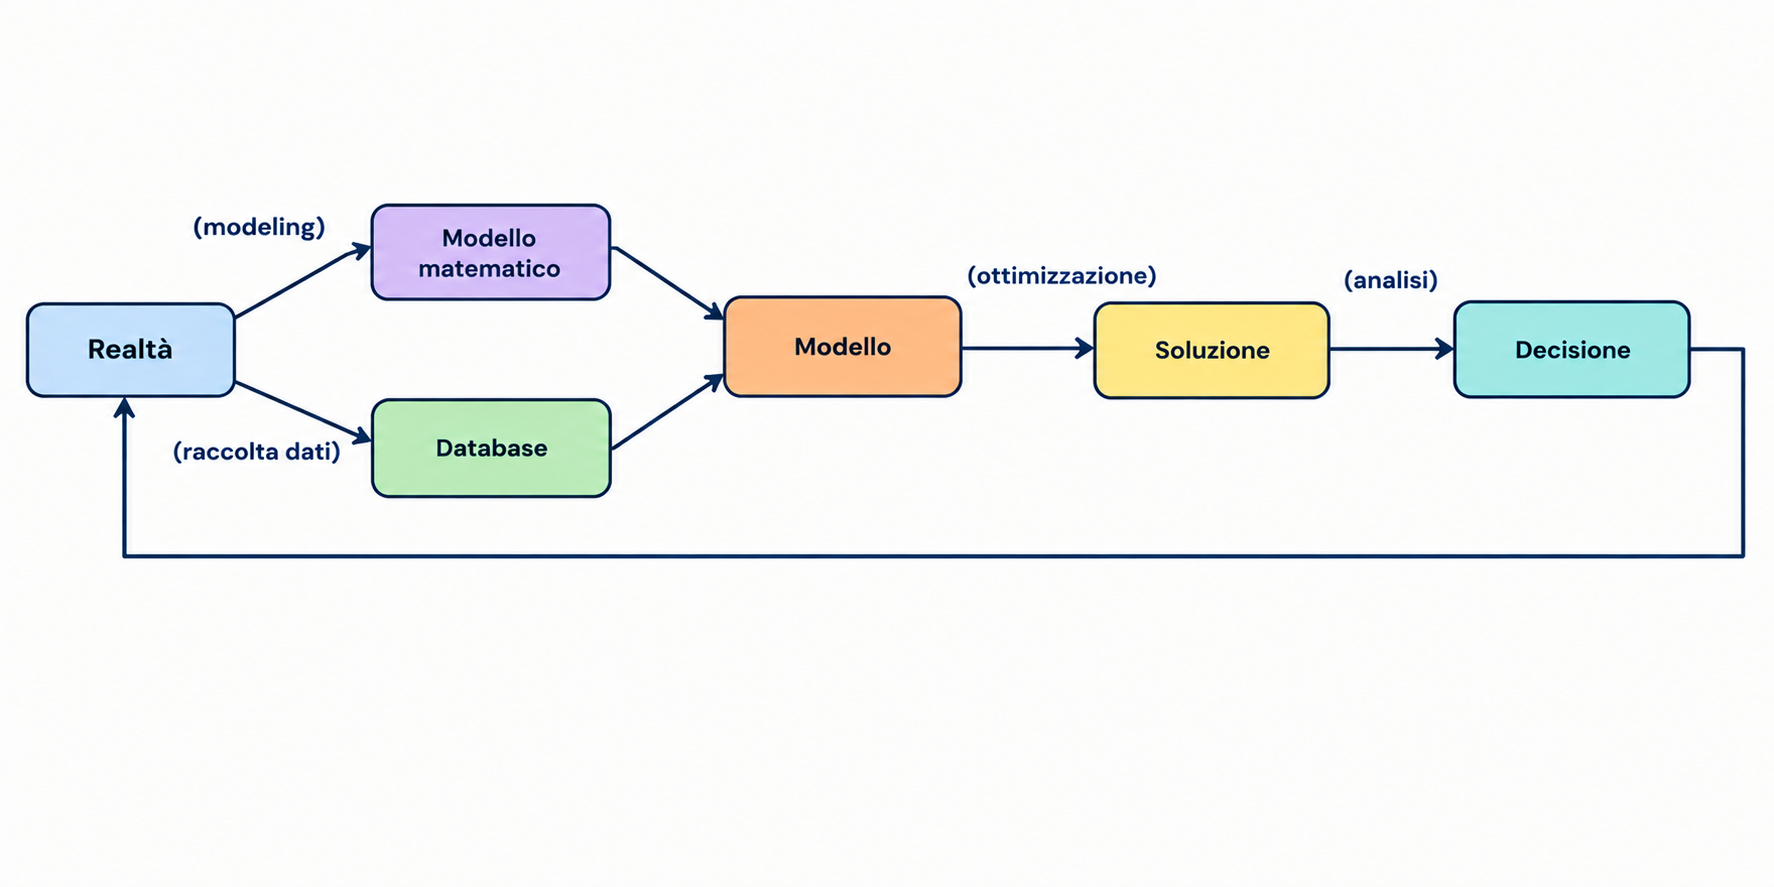
\includegraphics[width=\textwidth]{images/Diagram.png}
    \caption{Processo decisionale - diagramma a blocchi.}
    \label{fig:diagram}
\end{figure}
\begin{itemize}
    \item \textbf{Realtà:} si parte da un problema, una realtà di interesse.
    \item \textbf{Database:} si raccolgono i dati necessari per descrivere il problema e trovare una soluzione.
    \item \textbf{Modello matematico:} si convertono informazioni in variabili e dati matematici, come vincoli e funzione obiettivo.
    \item \textbf{Modello:} i dati e il modello matematico vengono combinati per ottenere i valori effettivi del problema e creare quindi il modello del problema specifico.
    \item \textbf{Soluzione:} trovata attraverso le operazioni di ottimizzazione del modello specifico.
    \item \textbf{Decisione:} una volta analizzata e processata la soluzione si decide come procedere.
\end{itemize}
Il processo decisionale è ciclico perchè la decisione viene applicata alla realtà, che può presentare nuovi problemi.
\section{Modelli di ottimizzazione}
Un \textbf{modello di ottimizzazione} è una rappresentazione matematica di un problema decisionale.\\
Un modello tale serve a risolvere un problema di ottimizzazione e per farlo utilizza questi:
\begin{itemize}
    \item \textbf{Funzione Obiettivo:} rappresenta ciò che vogliamo massimizzare o minimizzare (profitto, produzione...)
    \item \textbf{Variabili decisionali:} incognite del modello
    \item \textbf{Vincoli:} rappresentano le limitazioni del problenma, come il budget.
    \item \textbf{Parametri:} valori fissi, influenzano funzione obiettivo e vincoli ma non possono essere modificati.
\end{itemize}

\subsection{Programmazione lineare e lineare intera}
I nostri modelli devono essere lineari.
\paragraph{Programmazione lineare:} se i vincoli e la funbzione obiettivo sono lineari e le variabili sono continue.
\paragraph{Programmazione lineare intera:} se i vincoli e la funzione obiettivo sono lineari e alcune delle variabili sono discrete (o \textbf{intere}).\\\\
Nei nostri modelli non si può:
\begin{itemize}
    \item Dividere o moltiplicare per variabili
    \item Utilizzare valori assoluti
\end{itemize}
Si possono solo utilizzare somme e moltiplicazioni o divisioni per parametri.

\subsection{Pianificazione della produzione (esempio)}
Osserviamo adesso un problema d'esempio per apprendere come trovare un modello di ottimizzazione e quindi una soluzione ottimizzata.
\subsubsection{Descrizione del problema}
La società Pintel deve pianificare la produzione della sua fabbrica di microprocessori. L'azienda possiede due diverse linee di prodotti: processori Pintium, venduti a 500 euro, ed i Coloron, venduti a 200 euro perche meno potenti, destinati ai consumer semplici.\\
L'impianto è in grado di realizzare 3000 "wafer" alla settimana, su ogni wafer trovano posto 500 coloron oppure 300 Pintium.\\
La resa di un wafer dipende dal tipo di processore:
\begin{itemize}
    \item Pintium: $50\%$
    \item Coloron: $60\%$
\end{itemize}
Ogni settimana si può mettere sul mercato un massimo di $400.000$ unità per evitare il calo dei prezzi per i Pintium, $700.000$ per i Coloron invece.\\
Si vuole capire quale quantità di ciascun modello bisonerebbe produrre settimanalmente per massimizzare il profitto.
\subsubsection{Inizializzazione}
Iniziamo con la preparazione dei nostri dati, vediamo le variabili:
\begin{itemize}
    \item $X_P$: numero di processori Pintium.
    \item $X_C$: numero di processori Coloron.
\end{itemize}
La funzione obiettivo è:
\[
maxZ = 500X_p + 200X_C
\]
I vincoli sono:
\[
\begin{cases}
    0 \leq X_P \leq 400.000\\
    0 \leq X_C \leq 700.000\\
    \frac{X_P}{300 \cdot 0,5} + \frac{X_C}{500 \cdot 0,6} \leq 300
\end{cases}
\]

\subsubsection{Traduzione in grafico e soluzione}
Per disegnare il grafico corrispondente inanzitutto è consigliato semplificare i dati comprimendoli (per esempio quantità di centinaia o migliaia).\\
Bisogna rappresentare i vincoli e ridurre il dominio, trovando lo \textbf{spazio soluzione}.\\
Una volta fatto questo, bisogna massimizzare la funzione obiettivo con l'utilizzo del gradiente, in questo caso:
\[
\nabla z = (500,200)
\]
La soluzione consiste nell'ultimo punto in cui il gradiente, scorrendo verso destra, rimane nel dominio.
\subsection{Possibili soluzioni dei problemi di ottimizzazione}
Un problema di ottimizzazione può avere diversi tipi di soluzione, tra cui:
\begin{itemize}
    \item \textbf{Un'unica soluzione ottima:} singola soluzione perfetta.
    \item \textbf{Soluzioni infinite:} non esiste una singola soluzione ottima.
    \[
    z = 10 \rightarrow \text{ tutto lo spazio soluzione.}
    \]
    \begin{center}
        Punti infiniti, soluzioni infinite.
    \end{center}
    \item \textbf{Problema illimitato:} spazio soluzione non chiuso (superiormente o inferiormente), non esiste una soluzione, bensì è $\infty$.
    \item \textbf{Nessuna soluzione:} lo spazio soluzione è vuoto.
\end{itemize}

\section{Tecniche di modellazione dei problemi}
Alcuni problemi possono essere molto complessi, è quindi necessario sapere come modellarli per renderli risolvibili.
\subsection{Il problema della fonderia (esempio)}
\subsubsection{Descrizione del problema}
Una fonderia deve produrre 1000 pezzi del peso ciascuno di $1$ kg. Il ferro con cui tali pezzi sono fatti dovrà contenere almeno il $3,25\%$ e al più $5,5\%$ di silicio, inoltre dovrà contenere al meno lo $0,45\%$ di manganese. Per il mix, sono disponibili tre tipi di materiale ferroso con le caratteristiche in foto.\\
Inoltre, si può aggiungere direttamente manganese al costo di $10£/kg$.\\\\
Si vuole determinare il piano di produzione che minimizza il costo del materiale utilizzato.
\begin{table}[h]
    \centering
    \begin{tabular}{cccc}
        \hline
        Materiale ferroso & 1 & 2 & 3 \\
        \hline
        Silicio (\%)    & 4,00  & 1,00  & 0,60  \\
        Manganese (\%)  & 0,45  & 0,50  & 0,40  \\
        Costo (£/kg)    & 0,025 & 0,030 & 0,018 \\
        \hline
    \end{tabular}
    \caption{Composizione e costo dei materiali}
    \label{tab:composizione_costo}
\end{table}
\subsubsection{Inizializzazione}
Iniziamo col definire delle costanti:
\begin{itemize}
    \item $n = 4$, numero dei materiali.
    \item $K = 1000$, numero di pezzi da produrre.
    \item $e_i$, costo del materiale $i$.
    \item $s_i$, percentuale di silicio del materiale $i$.
    \item $m_i$, percentuale di manganese del materiale $i$.
    \item $s,\overline{S}$, percentuale minima e massima di silicio.
    \item $m$, percentuale minima di manganese.
\end{itemize}
Iniziamo con le variabili:
\begin{itemize}
    \item \textbf{$X_1$}: materiale $1$
    \item \textbf{$X_2$}: materiale $2$
    \item \textbf{$X_3$}: materiale $3$
    \item \textbf{$X_4$}: manganese extra
\end{itemize}
Poi i vincoli:
\[
\begin{cases}
    X_1, X_2, X_3, X_4 \geq 0\\
    3,25 \cdot 1000 \leq 4 \cdot X_1 + X_2 + 0,6 \cdot X_3 \leq 5,5 \cdot 1000\\
    0,45 \cdot X_1 + 0,5 \cdot X_2 + 0,4 \cdot X_3 + 100 \cdot X_4 \geq 0,45 \cdot 1000
\end{cases}
\]
La funzione obiettivo invece è:
\[
minZ = 0,25 \cdot X_1 + 0,03 \cdot X_2 + 0,018 \cdot X_3 + 10 \cdot X_4
\]
Adesso la fonderia vuole aggiungere un nuovo vincolo al mix di fusione: adesso il materiale 1 rispetto ai materiali ferrosi utilizzati nella fusione deve rappresentare almeno il 20\%. Scriviamolo subito e aggiorniamo i vincoli:
\[
\begin{cases}
    X_1, X_2, X_3, X_4 \geq 0\\
    3,25 \cdot 1000 \leq 4 \cdot X_1 + X_2 + 0,6 \cdot X_3 \leq 5,5 \cdot 1000\\
    0,45 \cdot X_1 + 0,5 \cdot X_2 + 0,4 \cdot X_3 + 100 \cdot X_4 \geq 0,45 \cdot 1000\\
    \frac{X_1}{X_1 + X_2 + X_3} \geq 0,20
\end{cases}
\]
Questo non va bene perchè non è lineare, spostiamo il denominatore a destra:
\[
\begin{cases}
    X_1, X_2, X_3, X_4 \geq 0\\
    3,25 \cdot 1000 \leq 4 \cdot X_1 + X_2 + 0,6 \cdot X_3 \leq 5,5 \cdot 1000\\
    0,45 \cdot X_1 + 0,5 \cdot X_2 + 0,4 \cdot X_3 + 100 \cdot X_4 \geq 0,45 \cdot 1000\\
    X_1 \geq 0,20 \cdot (X_1 + X_2 + X_3)
\end{cases}
\]
\subsubsection{Un problema difficile: generalizzazioe}
Il problema è molto complesso ed è necessario semplificarlo / generalizzarlo.\\
Ecco come si aggiornano i vincoli per renderli generali:
\[
min = \sum_{i = 1}^{n} c_i \cdot X_i
\]
\[
min = \sum_{i = 1}^{n} X_i = K
\]
\[
s \cdot K \leq min = \sum_{i = 1}^{n - 1} s_i \cdot X_i \leq \overline{S} \cdot K
\]
\[
\sum_{i = 1}^{n} m_i \cdot X_i \geq m \cdot K
\]
\[
x_i \geq 0, \forall i = \{1,\ldots,n\}
\]
Spiegando riga per riga:
\begin{enumerate}
    \item La funzione obiettivo corrisponde alla somma dei costi di ogni pezzo prodotto.
    \item La somma di tutti i pezzi prodotti corrisponde alla quantità di pezzi da produrre.
    \item La quantità di silicio totale in ogni pezzo deve rispettare i limiti massimi e minimi specificati prima. L'ultimo materiale è escluso perchè è puro manganese.
    \item La quantità di manganese totale in ogni pezzo prodotto deve rispettare la soglia minima specificata prima.
    \item La variabile che conta i pezzi per un qualsiasi materiale è non negativa.
\end{enumerate}


\section{Variabili binarie}
\subsection{Problema dello zaino (Esempio)}
\subsubsection{Descrizione del problema}
Un investitore dispone di un capitale limitato B da destinare a una serie di $n \in N$ progetti di investimento.\\
Ogni progetto è caratterizzato da:
\begin{itemize}
    \item un \textbf{costo di investimento} $c_i$, per ogni progetti $i \in I = \{1,\ldots,n\}$.
    \item un \textbf{rendimento atteso} $w_i$, per ogni progetto $i \in I = \{1,\ldots,n\}$.
\end{itemize}
L'investitore deve decidere quali progetti finanziare per massimizzare il rendimento atteso complessivo dato il capitale disponibile.\\
I parametri sono tutti non negativi (dato che è specificato nella descrizione, non deve essere un vincolo, ma un controllo preliminare).
\subsubsection{Inizializzazione}
Partiamo con le costanti:
\begin{itemize}
    \item B: capitale.
    \item $n$: progetti.
    \item $c_i$: costo del progetto $n_i$ con $i \in I = \{1,\ldots,n\}$
    \item $w_i$: rendimento del progetto $n_i$ con $i \in I = \{1,\ldots,n\}$.
\end{itemize}
Ora le variabili:
\begin{itemize}
    \item $X_i$: variabile binaria, \textbf{(1)} se prendo il progetto, \textbf{(0)} altrimenti.
\end{itemize}
Ora la funzione obiettivo:
\[
maxZ = \sum_{i \in I}^{} w_i \cdot X_i
\]
In questo modo la funzione conta solo i progetti scelti per massimizzare la soluzione.\\
Adesso guardiamo i vincoli:
\[
\begin{cases}
    \sum_{i \in I}^{} c_i \cdot X_i
    X_1 = \{0,1\}
\end{cases}
\]
\subsubsection{Rappresentazione relazioni logiche}
Si aggiungono nuovi vincoli:
\begin{enumerate}
    \item Ci sono due progetti in competizione (A,B). L'investitore intende finanziare esattamente uno tra essi.
    \item E se volesse finanziarne al minimo uno?
    \item E se volesse finanziarne al massimo uno?
\end{enumerate}
Ecco come si rappresentano:
\begin{enumerate}
    \item $X_A + X_B = 1$
    \item $X_A + X_B \geq 1$
    \item $X_A + X_B \leq 1$
\end{enumerate}
Adesso, consideriamo che se si investe in A, allora si investe in B, ma se non si investe in A non è necessario investire in C.\\
Ecco come si rappresenta:
\[
X_A \leq X_C
\]
Infine:
\begin{itemize}
    \item Se finanziamo A e B, allora finanziamo anche C.
    \item Si può finanziare il progetto C solo se si finanziano A e B.
\end{itemize}
Si ha una doppia implicazione:
\[
\begin{cases}
    \frac{X_A + X_B}{2} \leq X_C\\
    X_C = \frac{X_A + X_B}{2}
\end{cases}
\]
La prima condizione si annulla e quindi:
\[
X_C \geq X_A + X_B - 1
\]
\end{document}